\chapter{System Evaluation}
\section{What went wrong}
Upon completion of this project, there were a few things that stood out to us during development and in the final product. To start, one thing we did not anticipate is how difficult working with packages can be. For example, a feature that we really wanted to implement was the saving of the QR code feature on the QR code generation screen. We followed the documentation, we had permissions being requested on the screen of the simulator but then nothing happened after that, the QR code never appeared in our camera roll. We assumed that maybe this was because we were using the simulator and not our device. So when we tried to build the project onto our iPhone, XCode displayed multiple errors saying as seen in the image below.
\begin{center}
    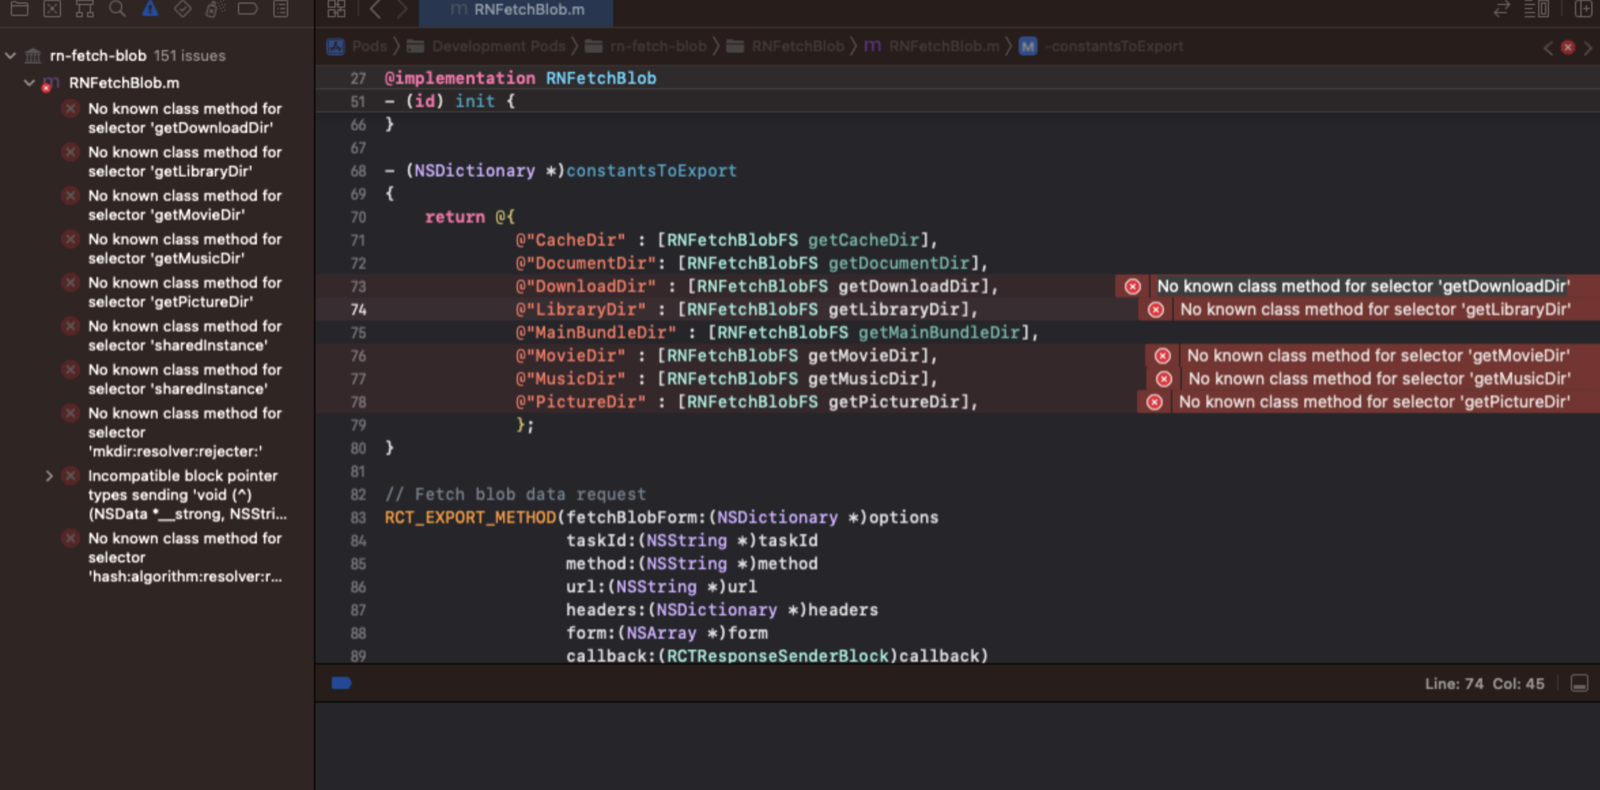
\includegraphics [scale=0.50]{atu-computing-latex-template/images/getDownloadDir.png}
\end{center}
We spent a lot of valuable time trying to implement this feature and we couldn't get it working. We were disappointed in this as we really would have liked to have that feature working. A way around this is that because the app is running on a mobile device, the user could screenshot the QR code. We were not able to find a fix to this issue and all we could find out is that the issue was due to the package 'react-native fetch-blob' that was being installed my NPM did included the methods but XCode for an unknown reason wouldn't pick up on them. Speaking XCode, something we found frustrating were the build times and the fact that we had to 'Sign Off' on every build as some modules required this but XCode would forget that we signed off every time we made a change to the project meaning we had to build our app twice, every time.

Another feature we really wanted to have was to be able to receive verification codes via SMS. AWS Amplify has this in their set of methods and we had this feature nearly working. When creating the account, the user is meant to receive a verification code. We logged this process to the console to test it and it was logging correctly with no error messages indicating to us that it was working but we never received any verification code. We tried with multiple phone numbers on different networks, checked over our configuration on AWS Amplify and everything seemed fine. In the end we settled for email verification code's. We would have preferred SMS but as long as the user can receive a code its fine.
\begin{center}
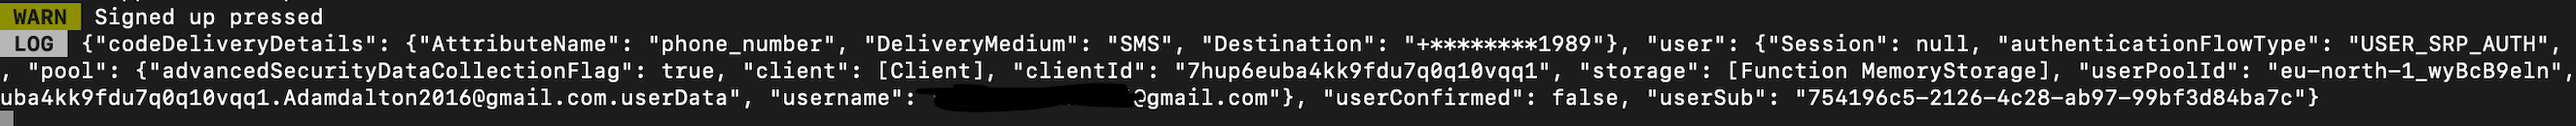
\includegraphics[scale=.30]{atu-computing-latex-template/images/codeLog.png}
\end{center}

Finally, one feature we didn't get to work fully was the user being able to reset their email address after they have signed in. The password update feature works fine but email one doesn't. We didn't get any errors when doing this to say that it didn't work, nothing in the console either. 

\section{What went well}
First off, we are happy with the features we were able to get working. The user can create an account and verify it, reset passwords, generate and scan QR codes, calculate tips etc. We for the most part completed the goal we set out to do. Secondly, from unit testing the project, we knew that the features worked individually and combining them together would work because apart from signing in, the main logic that was done was passing variables from one screen to another (e.g. the tip amount from the calculate tip screen to the QR Code scan screen) and so all we had to do was just figure out where do they fit in the overall projects structure. Overall, we are happy with the outcome of the project, especially because we had to learn a lot of new technologies to make this work.
\section{System Stability and Speed}
We can see from this table, that the build time is quite long. We tested it at 9 minutes and 4 seconds and that was from a clean build done through XCode. This included building, installing to iPhone and getting the server running. After that, any changes made required a much smaller build time. As for logging in, after entering a valid email address, was around 1.4 seconds. Opening the QR scanner was 1.5s and finally, scanning a QR code took around 1.4 seconds. 

The stability of the app is good. The only times an app crashed was when we were running the simulator and tried to open the camera which as we said is not allowed on iPhone simulators. We stress tested the app as well, running the app for a long time, going from screen to screen, entering values, closing the app and reopening. We didn't encounter any crashes when doing this on our device but as we said, crashes really only happened on the simulator.

\begin{table}[htp]
\centering
    \begin{tabular}{p{2cm}|p{2cm}|p{2cm}}
        \hline
        \multicolumn{3}{|c|}{System speed test} \\
        \hline
        Num & Test & Result \\
        \hline
        1 & Build Time & 9m 04s \\
        \hline
        2 & Change Screens & 0.87s \\
        \hline
        3 & Login Time & 1.87s \\
        \hline
        4 & Open QR & 1.5s \\
        \hline
        5 & Scan QR & 1.4s \\
        \hline
    \end{tabular}
    \caption{System speed test}
    \label{table:Stability}
\end{table}